\documentclass[problem]{mcs}

\begin{pcomments}
  \pcomment{MQ_expectHHH}
  \pcomment{similar to MQ_expectHH-TT}
  \pcomment{shorter variation of CP_consecutive_coin_flips}
  \pcomment{ARM 5/5/12}
\end{pcomments}

\pkeywords{
  expectation
  total_expectation
  probability_tree
  tree_model
}

%%%%%%%%%%%%%%%%%%%%%%%%%%%%%%%%%%%%%%%%%%%%%%%%%%%%%%%%%%%%%%%%%%%%%
% Problem starts here
%%%%%%%%%%%%%%%%%%%%%%%%%%%%%%%%%%%%%%%%%%%%%%%%%%%%%%%%%%%%%%%%%%%%%

\begin{problem}
A coin with probability $p$ of flipping Heads and probability $q
\eqdef 1-p$ of flipping tails is repeatedly flipped until three
consecutive Heads occur.  The outcome tree $D$ for this setup is
illustrated in Figure~\ref{HHHtree}.

    \begin{figure}
      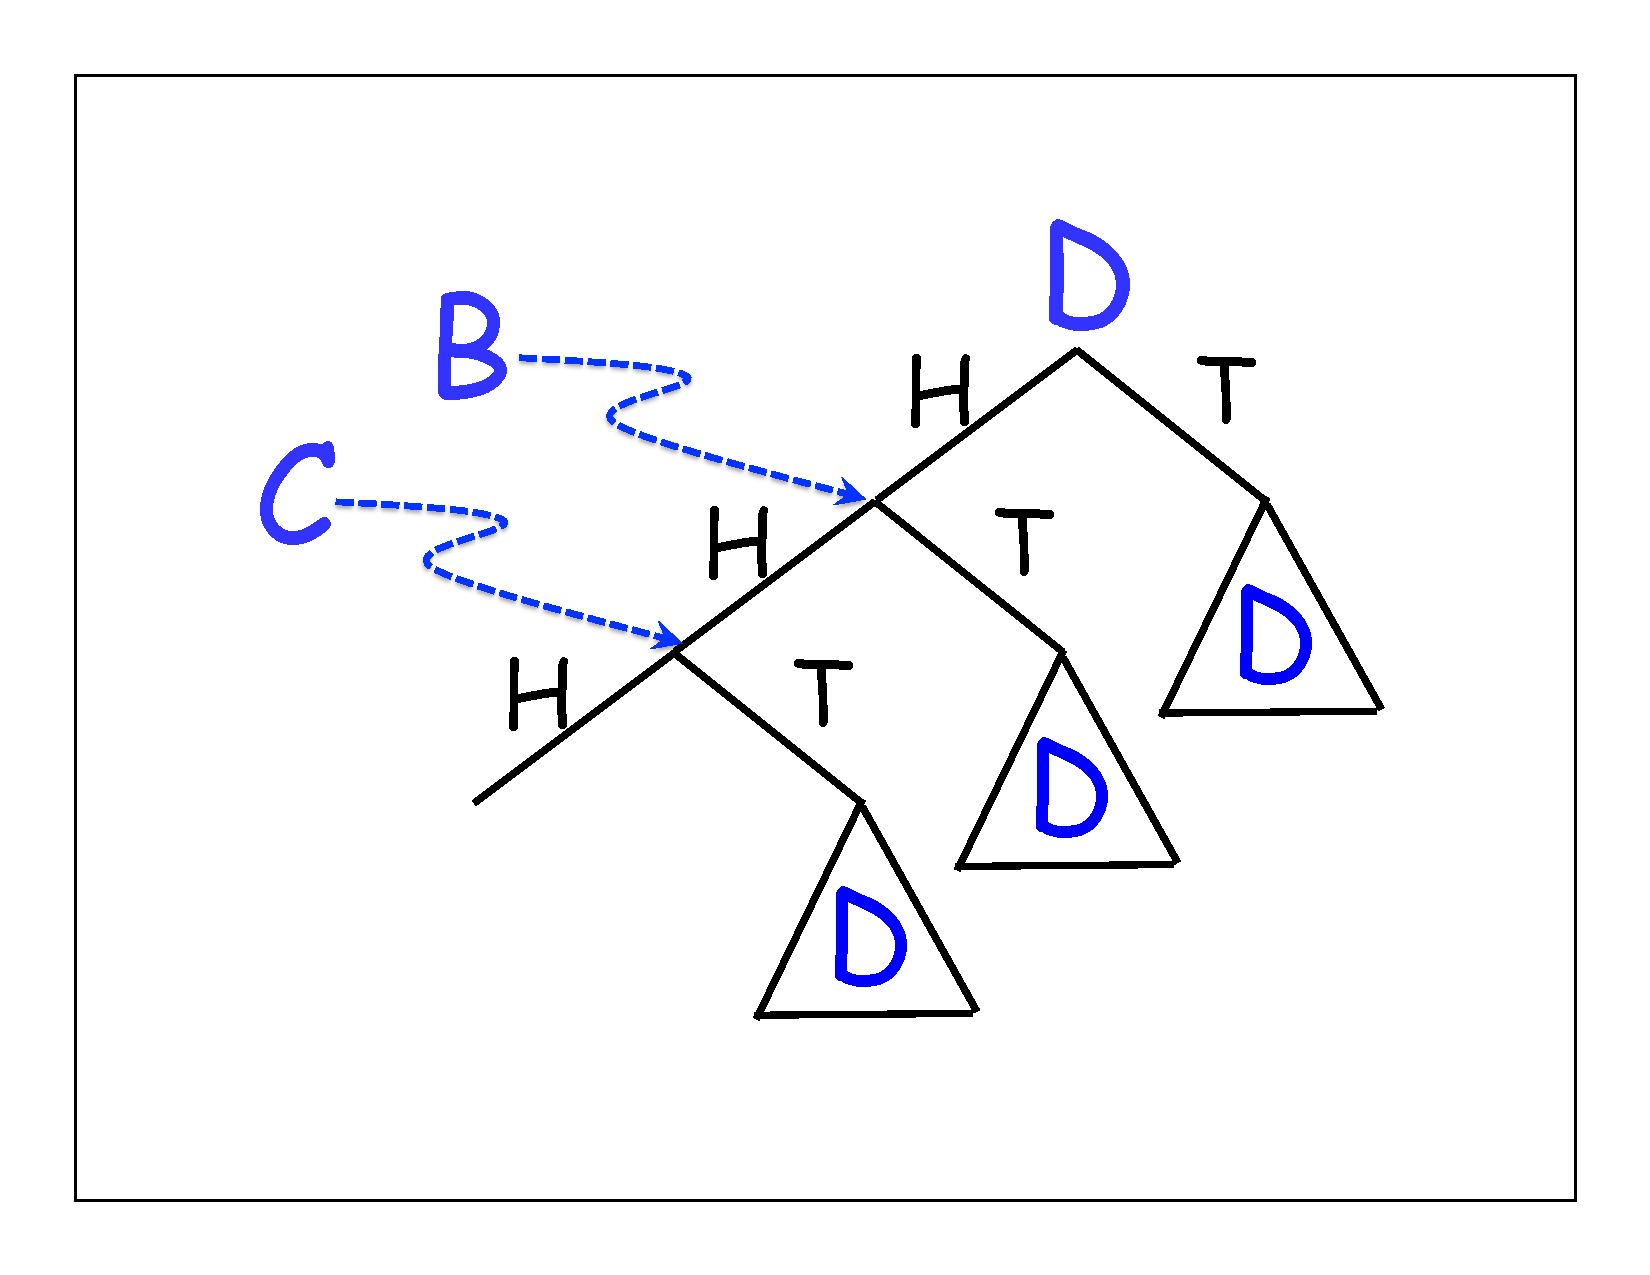
\includegraphics[width=3.5in]{HHHtree-frame}
     \caption{Outcome Tree for Flipping Until HHH}
     \label{HHHtree}
    \end{figure}

Let $e(S)$ be the expected number of flips starting at the root of
subtree $S$ of $D$.  So we're interested in finding $e(D)$.

\iffalse

Using the fact that the outcome tree $D$ for this setup can be
described as
\begin{align*}
D & \eqdef T\cdot D + H\cdot B\\
B & \eqdef T\cdot D + H \cdot C\\
C & \eqdef T\cdot D + H,
\end{align*}
\fi

Write a small system of equations involving $e(D), e(B)$, and $e(C)$
that could be solved to find $e(D)$.  \emph{You do \textbf{not} need
  to solve the equations.}

\begin{solution}
By the Total Expectation Rule, we have
\begin{align*}
e(D) & = q(1+ e(D)) + p(1+e(B)) = 1 + q\,e(D) + p\,e(B),\\
e(B) & = q(1+ e(D)) + p(1+e(C)) = 1 + q\,e(D) + p\,e(C),\\
e(C) & = q(1+ e(D)) + p(1+0)    = 1 + q\,e(D).
\end{align*}

A solution to these equations was not called for, but is easy to work
out.  Namely, substituting for $e(C)$, we get
\[
e(B) = 1 + q\,e(D) + p(1+ q\,e(D)) = 1 + p + q\,e(D)(1+p)
\]
and then substituting this expression for $e(B)$, we get
\begin{align*}
e(D) & = 1 + q\,e(D) +p(1+p+q\,e(D)(1+p))\\
     & = 1+p+p^2 + q\,e(D)(1+p+p^2)\\
     & = (1+p+p^2)(1+q\,e(D))\\
     & = \frac{1-p^3}{q}(1+q\,e(D))\\
     & = (1-p^3)\paren{\frac{1}{q}+e(D)}
\end{align*}
so
\[
e(D)p^3  = \frac{1-p^3}{q}
\]
and
\[
e(D) = \frac{1-p^3}{qp^3}.
\]
For $p=1/2$, this would be 14.

\iffalse
Sanity check using Wald's Theorem: the expected number of flips is
\[
\frac{q+2pq+3p^2}{p^3}\ .
\]
\fi

\end{solution}

\end{problem}


%%%%%%%%%%%%%%%%%%%%%%%%%%%%%%%%%%%%%%%%%%%%%%%%%%%%%%%%%%%%%%%%%%%%%
% Problem ends here
%%%%%%%%%%%%%%%%%%%%%%%%%%%%%%%%%%%%%%%%%%%%%%%%%%%%%%%%%%%%%%%%%%%%%
